\documentclass{acm_proc_article-sp}

\usepackage[utf8]{inputenc}
\usepackage[T1]{fontenc}

\usepackage[activate=compatibility]{microtype}

% autoref command
\usepackage[pdftex,urlcolor=black,colorlinks=true,linkcolor=black,citecolor=black]{hyperref}
\def\sectionautorefname{Section}
\def\subsectionautorefname{Subsection}

\usepackage{enumitem}

% todo macro
\usepackage{color}
\newcommand{\todo}[1]{\noindent\textcolor{red}{{\bf \{TODO}: #1{\bf \}}}}

% listings and Verbatim environment
\usepackage{fancyvrb}
\usepackage{relsize}
\usepackage{listings}
\usepackage{verbatim}
\newcommand{\defaultlistingsize}{\fontsize{8pt}{9.5pt}}
\newcommand{\inlinelistingsize}{\fontsize{8pt}{11pt}}
\newcommand{\smalllistingsize}{\fontsize{7.5pt}{9.5pt}}
\newcommand{\listingsize}{\defaultlistingsize}
\RecustomVerbatimCommand{\Verb}{Verb}{fontsize=\inlinelistingsize}
\RecustomVerbatimEnvironment{Verbatim}{Verbatim}{fontsize=\defaultlistingsize}
\lstset{frame=lines,captionpos=b,numberbychapter=false,escapechar=§,
        aboveskip=0.5em,belowskip=0em,abovecaptionskip=0em,belowcaptionskip=0em,
framexbottommargin=-1em,
        basicstyle=\ttfamily\listingsize\selectfont}

% use Courier from this point onward
\let\oldttdefault\ttdefault
\renewcommand{\ttdefault}{pcr}
\let\oldurl\url
\renewcommand{\url}[1]{\inlinelistingsize\oldurl{#1}}

\lstdefinelanguage{JavaScript}{
  keywords={push, typeof, new, true, false, catch, function, return, null, catch, switch, var, if, in, while, do, else, case, break},
  keywordstyle=\bfseries,
  ndkeywords={class, export, boolean, throw, implements, import, this},
  ndkeywordstyle=\color{darkgray}\bfseries,
  identifierstyle=\color{black},
  sensitive=false,
  comment=[l]{//},
  morecomment=[s]{/*}{*/},
  commentstyle=\color{darkgray},
  stringstyle=\color{red},
  morestring=[b]',
  morestring=[b]"
}

% linewrap symbol
\definecolor{grey}{RGB}{130,130,130}
\newcommand{\linewrap}{\raisebox{-.6ex}{\textcolor{grey}{$\hookleftarrow$}}}

% more pleasing quote environment
\usepackage{tikz}
\newcommand*{\openquote}{\tikz[remember picture,overlay,xshift=-7pt,yshift=1pt]
     \node (OQ) {\fontfamily{fxl}\fontsize{16}{16}\selectfont``};\kern0pt}
\newcommand*{\closequote}{\tikz[remember picture,overlay,xshift=2pt,yshift=-4.5pt]
     \node (CQ) {\fontfamily{fxl}\fontsize{16}{16}\selectfont''};}
\renewenvironment{quote}%
{\setlength{\parindent}{1cm}\par\openquote}
{\closequote\vspace{-4.5pt}
}

% bullet numbers
\usepackage{tkz-graph}
\usetikzlibrary{matrix,arrows,decorations.pathmorphing,shapes}
\newcommand{\dobulletnumber}[1]{\node[circle,text=white,fill=gray,anchor=west,inner sep=1pt] {\sffamily #1}}
\newcommand{\bulletnumber}[1]{\tikz[baseline=-2.5,overlay]\dobulletnumber{#1};}
\newcommand{\bulletref}[1]{\tikz[baseline=-2.5]\dobulletnumber{\fontsize{8}{8}\selectfont#1};}

\hyphenation{DBpedia RESTdesc}

% \def\baselinestretch{0.98}

\begin{document}

\title{Enabling On-the-Fly Video Shot Detection on YouTube\\ and Crowdsourcing In-Video Hot Spot Identification}

\numberofauthors{7}\author{
\alignauthor
Thomas Steiner\\
	\affaddr{Google Germany GmbH}\\
	\affaddr{ABC-Str. 19}\\
	\affaddr{20354 Hamburg, Germany}\\
	\email{tomac@google.com}
\alignauthor
Ruben Verborgh\\
	\affaddr{Ghent University -- IBBT, ELIS}\\
	\affaddr{Multimedia Lab}\\
	\affaddr{Gaston Crommenlaan 8/201}\\
	\affaddr{9050 Ghent, Belgium}\\
	\email{ruben.verborgh@ugent.be}
\alignauthor	
Michael Hausenblas
	\affaddr{DERI, NUI Galway}
	\affaddr{IDA Business Park}
	\affaddr{Lower Dangan Galway, Ireland}
	\email{michael.hausenblas@deri.org}
\and	
\alignauthor	
Rapha\"{e}l Troncy\\
       \affaddr{EURECOM}\\
       \affaddr{Sophia Antipolis}\\
       \affaddr{France}\\
       \email{raphael.troncy@eurecom.fr}
\alignauthor
Joaquim Gabarr\'o Vall\'es\\
	\affaddr{Universitat Polit\`{e}cnica}\\
	\affaddr{de Catalunya}\\
	\affaddr{Department LSI}\\
	\affaddr{08034 Barcelona, Spain}\\
	\email{gabarro@lsi.upc.edu}
\alignauthor
Rik Van de Walle\\
	\affaddr{Ghent University -- IBBT, ELIS}\\
	\affaddr{Multimedia Lab}\\
	\affaddr{Gaston Crommenlaan 8/201}\\
	\affaddr{9050 Ghent, Belgium}\\
	\email{rik.vandewalle@ugent.be}
}
\additionalauthors{Arnaud Brousseau (intern at Google Germany GmbH and EURECOM M.Sc. student at the time of writing), email: \texttt{arnaud.brousseau@gmail.com}.}
\maketitle
\begin{abstract}
Video shot detection is the processor-intensive task of splitting a video into continuous shots, with hard or soft cuts as the boundaries. In this paper, we present a client-side on-the-fly approach to this challenge based on modern HTML5-enabled Web APIs. We show how using browser extensions video shot detection can be seamlessly embedded into video platforms like YouTube. We then explain how the generated set of shots of a video drives crowdsourced identification of ``hot spots'', interesting shots watched by many viewers.
%We evaluate our approach based on a set of videos that were manually split into shots and annotated with hot~spots, indicating the potential of this technique.
A screencast of our approach is available on YouTube\footnote{\todo{Provide URL of screencast}}.
\end{abstract}

\category{H.x.y}{Example Category}[\todo{Find proper categories}]

\terms{\todo{Find proper terms}}

\keywords{\todo{Find proper keywords}}

%%%%%%%%% BODY TEXT
\section{Introduction}
Official press statistics~\cite{youtube:stats} from YouTube, one of the biggest online video platforms, state that more than 13 million hours of video were uploaded during 2010, and that 48 hours of video are uploaded every single minute. Given this huge amount of video content, it becomes evident that advanced search techniques are necessary in order to retrieve the few needles from the giant haystack. Closed captions allow for keyword-based in-video search, a feature announced in 2008~\footnote{\url{http://googlevideo.blogspot.com/2008/06/closed-captioning-search-options.html}}. Searching YouTube for a phrase like ``that's a tremendous gift'', a caption from Randy Pausch's famous last lecture \emph{Achieving Your Childhood Dreams}\footnote{\url{http://www.youtube.com/watch?v=ji5\_MqicxSo}}, reveals the video of his lecture. If no closed captions are available, nor can be automatically generated, keyword-based search is still available over tags, video descriptions, and titles. Presented with a potentially long list of results, preview thumbnails based on video still frames help users decide on the most promising result. YouTube uses an unpublished computer vision-based algorithm for the generation of smart thumbnails on YouTube and lets video owners choose one out of three automatically suggested thumbnails.

\begin{comment}
Until December 2008, the mechanism for the generation of such thumbnails has been simply the so-called 25/50/75 rule~\cite{youtuberule}, referring to points in the video index. This led to creative abuse of the feature to artificially increase a video's click-through rate through strategic placement of, e.g., attractive women. Currently, YouTube uses an unpublished computer vision-based algorithm for the generation of smart thumbnails on YouTube~\cite{googleresearch}.
\end{comment}

In this paper, we introduce on-the-fly shot detection for YouTube videos together with in-video hot spots as a third means besides keyword-based search and thumbnail preview for deciding on a video from the haystack. As a user starts watching a video, we detect shots in the video by visually analyzing its content. We do this with the help of a browser extension, i.e., the whole process runs dynamically on the client-side, using modern HTML5~\cite{w3c_html5} JavaScript APIs of the \texttt{<video>} and \texttt{<canvas>} elements. As soon as the shots have been detected, we offer the user the choice to quickly jump into a~specific shot by clicking on a~representative still frame. \autoref{fig:screenshot} shows the seamless integration of the detected shots into the YouTube website enabled by the browser extension. We refer to shots that receive clicks as \emph{hot spots}. Clicks on hot spots are tracked using a standard Web analytics service, which allows as to suggest more accurate entry points to videos in the longterm. The main contributions of this paper are the browser extension itself, the hot~spot-enabled more accurate video thumbnail selection, and improved video navigability by shot navigation.

\begin{comment}
The remainder of this paper is structured as follows: \autoref{sec:related-work} presents related work in the fields of shot boundary detection and semantic enrichment of user-generated metadata on YouTube, \autoref{sec:details-of-algo} explains our shot detection algorithm in detail, \autoref{sec:implementation} outlines the implementation details of our browser extension, \autoref{sec:evaluation} shows an evaluation of first preliminary results. Finally, \autoref{sec:future-work-conclusion} gives an outlook on future work and ends the paper with a~\mbox{conclusion}.
\end{comment}

\begin{figure}
\begin{center}
   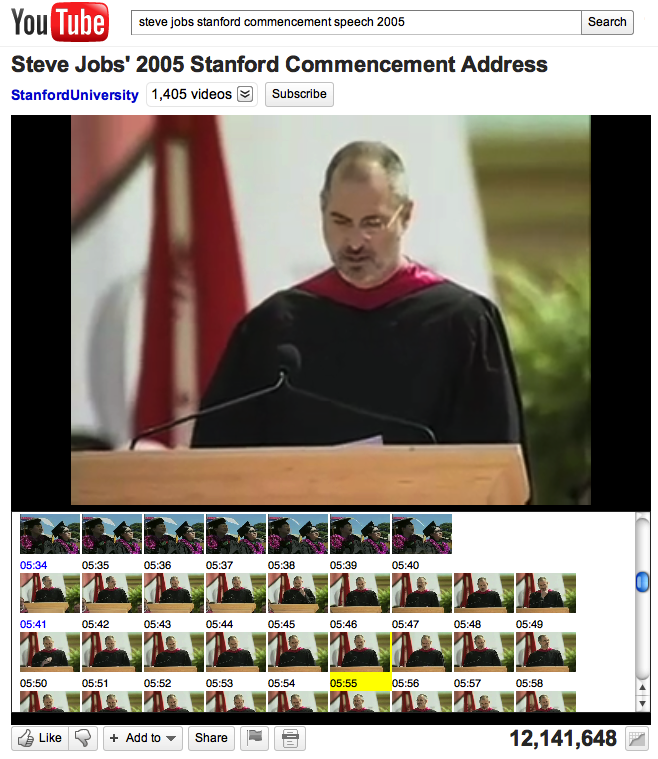
\includegraphics[width=0.85\linewidth]{./resources/stevejobs.png}
\end{center}
   \caption{Screenshot of the browser extension running on YouTube, showing different detected shots.}
\label{fig:screenshot}
\end{figure}

\section{Related Work} \label{sec:related-work}
Video fragments consist of shots, which are sequences of consecutive frames from a single viewpoint, representing a continuous action in time and space. The topic of shot boundary detection has already been described extensively in literature. While some specific issues still remain (notably gradual transitions and false positives due to large movement or illumination changes), the problem is considered resolved for many cases~\cite{Hanjalic2002, Yuan2007}. The contribution of our approach is that it is entirely Web-based and on-the-fly, which introduces interesting new challenges that traditional approaches do not have to cope with. A major issue is the uncertain streaming speed, where traditional approaches have immediate access to the video file on disk. An additional challenge is the unknown video codec and key frame distribution of the target videos, which -- together with streaming speed issues -- makes exact frame-wise video navigation impossible. Below, we present an overview of several well-known categories of shot detection techniques.

\emph{Pixel comparison methods}~\cite{Hampapur1994, Zhang1993} construct a discontinuity metric based on differences in color or intensity values of corresponding pixels in successive frames. This dependency on spatial location makes this technique very sensitive to (even global) motion. Various improvements have been suggested, such as prefiltering frames~\cite{Zhang1995}, but pixel-by-pixel comparison methods proved inferior in the end and have steered research towards other directions.

A related method is \emph{histogram analysis}~\cite{Smeaton1999}, where changes in frame histograms are used to justify the boundaries of shots. Their insensitivity to spatial information within a frame makes histograms less prone to partial and global movements in a shot. We can argue as a drawback that even visually very dissimilar frames can have similar overall histograms. For example, different shots in the same shot can be difficult to distinguish because of similar color information.

As a compromise, a third group of methods consists of a \emph{trade-off between the above two techniques}~\cite{Ahmed1999}. Different histograms of several, non-overlapping blocks are calculated for each frame, thereby categorizing different regions of the image with their own color-based, space-invariant fingerprint. The results are promising, while computational complexity is kept to a minimum, which is why we have chosen a variation on this approach in this paper.

Other approaches to shot boundary detection include the \emph{comparison of mean and standard deviations} of frame intensities~\cite{Lienhart1999}. Detection using other features such as edges~\cite{Zabih1995} and motion~\cite{Bouthemy1997} have also been proposed. However, Gargi \emph{et~al.}\ have shown that these more complex methods do not necessarily outperform histogram-based approaches~\cite{Gargi2000}. A detailed comparison can be found in Yuan~\emph{et~al.}~\cite{Yuan2007}. 

\section{Shot Detection Algorithm} \label{sec:details-of-algo}
In this Section, we discuss our shot detection algorithm, which falls in the category of histogram-based algorithms.  Since visually dissimilar video frames can have similar overall histograms, we also take local histograms into account. 
We therefore split video frames in freely configurable rows and columns, i.e., lay over a grid of tiles over the frames. The user interface (\autoref{fig:algorithm}) currently allows for anything from $\mathit{1} \times \mathit{1}$ to $\mathit{20} \times \mathit{20}$ layouts. For each step we examine a frame $\mathit{n}$ and its direct predecessor frame $\mathit{n - 1}$.

Apart from the per-tile histogram average distance, the frame distance function further considers a freely configurable number of \emph{most different} and \emph{most similar} tiles. This is driven by the observation that different parts of a video have different intensities of color changes, dependent on the movements from frame to frame. The idea is thus to increase the influence of movements in the frame distance function, and to decrease the influence of permanence. In the debug view of our approach (\autoref{fig:algorithm}), red boxes indicate movements, while green boxes indicate permanence. In the concrete example, Steve Jobs' head and shoulders move as he talks, which can be clearly seen by the red boxes in the particular tiles. Additional movements come from a swaying flag on the left, and a plant on the right. In contrast, the speaker desk, the white background, and the upper part of his body remain static, resulting in green boxes. For this example, we use a grid layout of $\mathit{20} \times \mathit{20}$ tiles (which implies $\mathit{numTiles} = \mathit{rows} \times \mathit{columns} = 400$), and a number $\mathit{nDiffSim}$ of most different or similar tiles of~$\mathit{133}$ (one third of all tiles). In consequence, we treat one third of all tiles as most different tiles, one third as normal tiles, and one third as most similar tiles. We apply boosting and limiting factors to the most different and most similar tiles respectively. We work with a $\mathit{boostingFactor}$ of~$\mathit{1.1}$, which slightly increases the impact of the most different tiles, and a $\mathit{limitingFactor}$ of~$\mathit{0.9}$, which slightly decreases the impact of the most similar tiles. The algorithm pseudo code can be seen in \autoref{code:algorithm}.

We define the average histogram distance between two frames $\mathit{n}$ and $\mathit{n - 1}$ as $\mathit{avgHisto}_{n}$. In a first step, we have examined the histogram distance data statistically, and experimentally found out that while the overall average frame distance $\mathit{avgDist}_{n}$, defined as: $$\mathit{avgDist}_{n} = \frac{1}{\mathit{numTiles}}\sum_{t=1}^{\mathit{numTiles}}\mathit{avgHisto}_{n_{t}}$$ is very intuitive to human beings, far more value lies in the standard deviation $\mathit{stdDev}_{n}$, based on the definition of the overall average frame distance $\mathit{avgDist}_{n}$: $$\sqrt{\frac{1}{\mathit{numTiles}}\sum_{t=1}^{\mathit{numTiles}}(\mathit{avgHisto}_{n_{t}} - \mathit{avgDist}_{n})^{2}}$$ We use the value of the standard deviation as a value for the shot splitting threshold~\cite{Lienhart1999} to come to very accurate shot splitting results. We found the boosting and limiting factors to have overall a positive quality impact on more lively videos, and a negative quality impact on more monotone videos. The results are found to be optimal if, after changing either the boosting or the limiting factors for the most similar or different tiles, the value of the shot splitting threshold is adapted to the new resulting standard deviation.

\begin{figure}
\begin{center}
   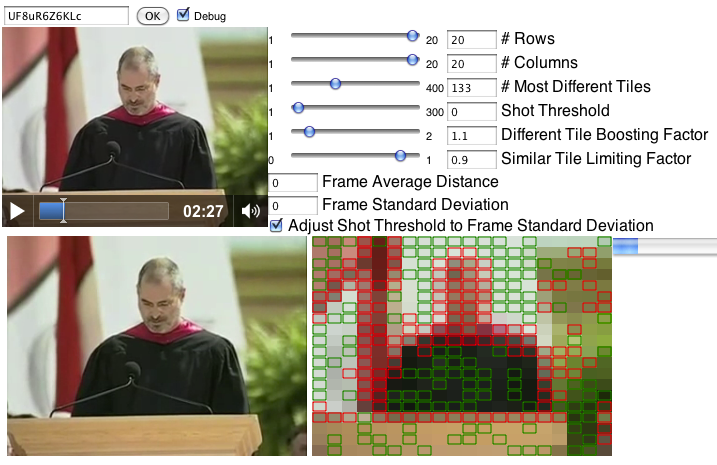
\includegraphics[width=0.9\linewidth]{./resources/algorithm.png}
\end{center}
   \caption{Debug view of the shot detection process. Red boxes highlight tiles with the most differences to the previous frame, green boxes those with most similarities.}
\label{fig:algorithm}
\end{figure}

\begin{lstlisting}[caption=Pseudocode of shot detection algorithm., label=code:algorithm, float]
for frame in frames
| n = frame.index  
| for tile in tiles of frame      
| | avgHisto[n][tile] = getTilewiseDiff()
|
| mostDiffTiles = getMostDiffTiles(avgHisto[n])
| mostSimTiles = getMostSimTiles(avgHisto[n])
|
| for tile in tiles of frame    
| | if tile in mostDiffTiles
| | | factor = boostingFactor
| | else if tile in mostSimTiles
| | | factor = limitingFactor
| | else
| | | factor = 1  
| | avgHisto[n][tile] = avgHisto[n][tile] * factor
| avgDist[n] = avg(avgHisto[n])
\end{lstlisting}

\section{Implementation Details} \label{sec:implementation}
Our shot detection algorithm is implemented in form of an extension for the Chrome browser. Chrome extensions are small software programs written in a combination of HTML, JavaScript, and CSS, which users can install to enrich their browsing experience. For this paper we focus on extensions based on so-called content scripts. Content scripts are JavaScript programs that run in the context of Web pages via dynamic code injection. By using the standard Document Object Model (DOM), they can read or modify details of the Web pages a user visits.

\begin{comment}
\paragraph{Google Analytics}
Google Analytics is Google's Web analysis solution allowing for detailed statistics about the visitors of a website. The software is implemented by adding an invisible snippet of JavaScript code on the to-be-tracked pages of a website. This code collects visitor data through a request for a specific $\mathit{1} \times \mathit{1}$ pixel image, during which the page and user data is reported back in the query part of the image's URL. In addition to that, the snippet sets a first party cookie on visitors' computers in order to store anonymous information such as the timestamp of the current visit, whether the visitor is a new or returning visitor, and the website the visitor came from.
\end{comment}

The complete video analysis process happens fully on the client side. We use HTML5 JavaScript APIs of the \texttt{<video>} and \texttt{<canvas>} elements. The extension is activated as soon as the user enters a page that matches the URL pattern \url{http://www.youtube.com/watch*}, i.e., YouTube video watch pages. By default, YouTube uses Flash-encoded videos that are not programmatically accessible from a JavaScript context, however, via an API used by the YouTube \texttt{<iframe>} embed code, we can retrieve the HTML5 versions of a video. In order to obtain a video still frame from the \texttt{<video>} element at the current video position, we use the \texttt{drawImage()} function of the 2D context of the \texttt{<canvas>} element, which as its first parameter accepts a \texttt{<video>} element. We then analyze the video frame's pixels tile-wise and calculate the histograms. The pitfall with this approach is that, in order to retrieve the tile-wise pixel data from the 2D context of the \texttt{<canvas>}, we need the \texttt{getImageData()} function to which the so-called Same Origin Policy~\cite{sameoriginpolicy} applies. This means that the \texttt{<canvas>} cannot use the video data directly  from YouTube, but has to use a proxied version on the same domain, which means that we have to temporarily store the video on a proxy server. For processing speed reasons, we currently limit our approach to a resolution of one second, i.e., for each analysis step seek the video in second-steps. We then calculate the frame distances as outlined in \autoref{sec:details-of-algo}. For each frame, we generate an \texttt{<img>} element with a base64-encoded data URI representation of the video frame's data that later gets injected into the DOM tree of YouTube, as can be seen in \autoref{fig:screenshot}. Each of the \texttt{<img>} elements has a registered JavaScript event handler that upon click triggers two actions: first, the video seeks to the corresponding time, and second, the frame is tracked as a hot spot in the video. We therefore use Google Analytics event tracking~\footnote{\url{http://code.google.com/apis/analytics/docs/tracking/eventTrackerGuide.html}}.
%A sample hot spot tracking event code snippet is shown in \autoref{code:event}.

\begin{comment}
\begin{lstlisting}[caption=JavaScript hot spot event tracking code snippet. The \texttt{\_gaq} object refers to the Google Analytics event tracking queue., label=code:event, float=t, language=JavaScript]
_gaq.push(['filmstrip._trackEvent', 
    'seek',        // event type
    'Bo2p82aTQzo', // video ID
    '64'           // time cue
]);
\end{lstlisting} 
\end{comment}

\section{Evaluation} \label{sec:evaluation}
Detecting shots on-the-fly in streaming video comes with its very own challenges. First, it is a question of streaming speed. We have to stream the same video twice in parallel: on the one hand the user-visible version, and on the other hand the version used in the background for the analysis process. Note that due to the Same Origin Policy~\cite{sameoriginpolicy} we are forced to stream two copies of the video, one from YouTube to the user, and one from YouTube to the proxy server where the shot detection algorithm runs. Especially with high-definition (HD) video this can be very demanding. We do not attach the background \texttt{<video>} element to the DOM tree to save some CPU cycles, however, the video still needs to be seeked to each frame in second-steps and be processed. Even on a high-end computer (our experiments ran on a MacBook Pro, Intel Core 2 Duo 2,66 GHz, 8 GB RAM), the process of analyzing and displaying in parallel a $\mathit{1280} \times \mathit{720}$ HD video of media type \emph{video/mp4; codecs="avc1.64001F, mp4a.40.2"} causes an average CPU load of about 70\%. The HTML5 specification states that \textit{``[\ldots] when the playback rate is not exactly 1.0, hardware, software, or format limitations can cause video frames to be dropped [\ldots]''}~\cite{whatwgvideo} in order to keep up with the stream. In practice, this causes the analysis environment to be far from optimal. In our experiments we differentiated between false positives, i.e., shot changes that were detected, but not existent, and misses, i.e., shot changes that were existent, but not detected. Our algorithm detected fewer false positives than misses, the reasons being gradual transitions and shots shorter than one second (below our detection resolution) for misses, and large movements in several tiles for false positives. Overall, we reached an accuracy of about 86\%, which is far from perfect, but given the mentioned challenges sufficient for our use cases. 

\begin{comment}
\subsection{Video Shot Detection}
With this rather lengthy preamble, in \autoref{table:results} we present some first preliminary results. The analysis settings for the experiment were as follows: $\mathit{rows} = 20$, $\mathit{columns} = 20$, $\mathit{nDiffSim} = 133$, $\mathit{boostingFactor} = 2.0$, $\mathit{limitingFactor} = 0.5$, $\mathit{shotThreshold} = \mathit{standardDeviation}$. We had two humans split 10 randomly selected videos into shots, and afterwards compared their shot classification with the automatically generated one. We counted \emph{matches} (humans and machine agreed), \emph{misses} (humans detected a shot change, the machine did not), and \emph{false positives} (machine detected a shot change, humans did not). 

\begin{table}
\begin{center}  
    \begin{tabular}{ | l | c | c | c |}
    \hline
    \textbf{Video ID} & \textbf{Matches} & \textbf{Misses} & \textbf{False Positives} \\ \hline
    \texttt{nCAZIVoE\_AQ} &  8 &  1 & 1 \\ \hline
    \texttt{9cZk267ezLw}  &  8 &  1 & 0 \\ \hline
    \texttt{vqVdm6zMmRc}  &  4 & 12 & 2 \\ \hline
    \texttt{kFAJ-XAF7oM}  &  5 &  3 & 1 \\ \hline
    \texttt{118fTtOKoc4}  & 10 &  9 & 3 \\ \hline
    \texttt{xyLHGlUN9rM}  & 16 &  2 & 8 \\ \hline
    \texttt{iqqLmdLecJw}  &  6 &  0 & 4 \\ \hline
    \texttt{5eIqe3tPczE}  &  5 &  0 & 4 \\ \hline
    \texttt{noeTBLB30ac}  &  9 &  3 & 0 \\ \hline
    \end{tabular}
\end{center}
\caption{Comparison of manual and automatic shot detection.}
\label{table:results}
\end{table}

Having a closer look at the source videos and interpreting these results, we can see that most misses are due to frame drops in the background analysis video, especially with HD video material. Given the preamble, this is not surprising. In addition to that, our human shot detectors counted rapid shot changes far beyond one-second-resolution, as for example in the Harry Potter movie trailer (\texttt{vqVdm6zMmRc}). Already by design, our approach cannot compete with this fine level of granularity, nor does it make sense trying to get there given our objectives of allowing for video hot spot-enabled more accurate video thumbnail selection, and improved video navigability by shot access. A more critical problem was that sometimes when a video could not be seeked to the desired time, the still frame remained static, an effect that for an unknown reason reproducibly occurred in the Sky News report video on Amy Winehouse's funeral (\texttt{iqqLmdLecJw}). This seems to be more a problem with the video encoding and the key frames rather than a problem in our code. 

\subsection{Hot Spot Identification}
We had two humans look at shot frames of 30 randomly selected videos and asked them to click on frames they found visually appealing. This resulted in overall just over 200 hot spots being tracked via Analytics. After analyzing the hot spots manually, we found that the humans used them in two ways: first, in a \emph{navigational way}, and second, in an \emph{interest-based way}. For the navigational way, the humans jumped either back to the beginning of the video (the trivial case), or skipped intros, which could be repeatedly observed in several videos, e.g., in the Kernkraft 400 -- Zombie Nation music video \texttt{(z5LW07FTJbI}) that has an seemingly annoying intro in the first 12 seconds. For the second interest-based category, the humans were attracted by promising frames, e.g., the fire-spitting dragon in the Harry Potter trailer at position 6 seconds, that both humans clicked twice, or the Fail Blog clip Responsible Sibling Fail (\texttt{kFAJ-XAF7oM}), where both humans repeatedly watched a poor kid get hit hard on the head by a soccer ball.

If we compared the detected hot spot video frames with the actually displayed YouTube video thumbnails, we observe room for improvement. Based on the human testers whom we first showed the videos, and then asked to decide on the most appropriate thumbnail from a set of the actual thumbnail and video frames from video hot spots reported by different users, in close to 90\% of the cases the testers decided for a video hot spot frame, and not for the YouTube selected thumbnail. 
\end{comment}

\section{Future Work and Conclusion} \label{sec:future-work-conclusion}

\begin{comment}
In this paper, we have first presented related work in the field of video shot boundary detection and the semantic enrichment of user-generated metadata on YouTube. In continuation, we have introduced our shot detection algorithm, and have outlined its implementation details regarding the two used tools (Analytics and Chrome extensions), and the extension's underlying HTML5 JavaScript APIs. Finally, we have evaluated our approach for video shot detection and hot spot identification.
\end{comment}

In a first step, future work will consist in improving the analysis speed by dynamically selecting lower quality analysis video files, given that videos are available in several resolutions (both LD and HD). We will check in how far analysis results differ for the various versions. In a second step, we will work on more advanced heuristics for the various user-definable options in the analysis process (\autoref{fig:algorithm}). While there is no optimal configuration for all types of videos, there are some key indicators to look out for, namely the standard deviation $\mathit{stdDev_{n}}$ and the overall average frame distance $\mathit{avgDist_{n}}$, both dependent on the values of $\mathit{boostingFactor}$, $\mathit{limitingFactor}$, $\mathit{rows}$, and $\mathit{columns}$. Interpreting early  results, there is evidence that low complexity settings are sufficient in most cases, i.e., a number of $\mathit{rows}$ and $\mathit{columns}$ higher than~$2$ does not necessarily lead to more accurate shot detection results. The same applies to the number of to-be-considered most different or similar tiles $\mathit{nDiffSim}$. We have even had cases where not treating those tiles differently at all, i.e., setting $\mathit{boostingFactor} = \mathit{limitingFactor} = 1$, led to better results.

Concluding, we have promising first results, especially with regards to hot spot identification, which in the future can serve for more accurate entry point suggestions in long videos, or enable skip marks in videos with intros. For the task of suggesting video thumbnails, a combined crowdsourced hot spot-based approach can lead to more accurate results than the current purely computer vision-based approach. For shot detection, some challenges remain, especially with the observed streaming speed-related issues. Nonetheless, when searching for a certain point in a video, the obtained results already allow for focused in-video navigation.

\begin{comment}
As a third step, we want to combine our approach with elements of the approaches of Choudhury \emph{et~al.}~\cite{Choudhury:YouTube}, Steiner and Hausenblas~\cite{semwebvid}, and Gao \emph{et~al.}~\cite{Gao:2009}. We are convinced of the joint power of low-level visual analysis and the high-level semantic text-based analysis. In a fourth step, we might consider proceeding with a server-side, rather than a client-side approach, albeit given the current YouTube upload rates~\cite{youtube:stats}, crowdsourced client-side processing seems a viable option, at least for the millions of hours of already existing video material.
\end{comment}

\section*{Acknowledgments}
The research activities as described in this paper were funded by Ghent University, the Interdisciplinary Institute for Broadband Technology (IBBT), the Institute for the Promotion of Innovation by Science and Technology in Flanders (IWT), the Fund for Scientific Research Flanders (FWO Flanders), and the European Union.
This work was partially supported by the European Commission under Grant No. 248296 FP7 \mbox{I-SEARCH} project.
%Joaquim Gabarr\'o is partially supported by TIN-2007-66523 (FORMALISM), and SGR 2009-2015 (\mbox{ALBCOM}).

\bibliographystyle{abbrv}
\bibliography{www2012}

\balancecolumns
\end{document}